\section*{\underline{TÍTULO DEL PROYECTO}}
Diseño, desarrollo e implementación de un sistema de gestión, seguimiento y obtención de indicadores relacionados a programas de formación.\\


\section*{\underline{OBJETIVO DEL PROYECTO}}
Objetivo general:\\

Contribuir, posibilitar y facilitar el seguimiento de los programas de formación e inclusión tecnológica para mujeres adolescentes mediante el desarrollo e implementación de un sistema de seguimiento, control y obtención de métricas para estos programas.\\

Objetivos específicos:
\begin{itemize}
	\item Identificar y permitir la visualización de indicadores relevantes y representativos que ayuden al seguimiento de los programas.
	\item Proporcionar un sistema de notificaciones que comunique a los distintos tipos de usuarios sobre eventos que puedan ser previamente configurados por ellos.
	\item Permitir la configuración de distintos perfiles con diferentes niveles de  privilegios para utilizar el sistema.\\
\end{itemize}


\section*{\underline{DESTINATARIOS}}
El Trabajo Final de Grado se realizará en el marco del proyecto UNDEX 775/2019 aprobado al Depto. de Computación e Informática de la Facultad de Ingeniería del CRUC IUA (Resolución 441/2019), en la convocatoria 2019 de UNDEF \textbf{\cite{ResolucionUndex}}. En dicho proyecto se desarrollará la estrategia a implementar mediante un sistema software para gestionar el seguimiento de los programas de capacitación tecnológica para favorecer la inclusión de la mujer. \\


\section*{\underline{BENEFICIOS ESPERADOS}}
\begin{itemize}
	\item Obtención de indicadores y métricas para toma de decisiones.
	\item Estandarización, limpieza y centralización del almacenamiento de la información de los cursos evitando pérdidas de la misma.
	\item Automatización de la carga de datos correspondiente a los cursos, lo que conlleva a un menor esfuerzo por parte de las personas encargadas de realizar estas tareas.
	\item Seguimientos de las alumnas participantes y de los programas.
	\item Facilidad de acceso a la información.\\
\end{itemize}


\section*{\underline{ESTUDIO TÉCNICO}}
\begin{itemize}
	\item Para el desarrollo del software se utilizaran 3 lenguajes de programación diferentes:
	\begin{itemize}
		\item Para el Backend se utilizaran los lenguajes Golang y Python.
		\item Para el Frontend se utilizara Javascript apoyándose en un framework llamado React también basado en Javascript.
	\end{itemize}
	\item Se utilizarán tanto Bases de Datos Relacionales como No Relacionales para el guardado de datos.
	\item Para desplegar el sistema se utilizará un servidor provisto por el CRUC IUA.\\
\end{itemize}



\section*{\underline{FORMULACIÓN Y VALORACIÓN DE ALTERNATIVAS}}
Para la detección de alternativas se basó en varios puntos importantes: Costo, almacenamiento de datos, posibilidad de relizar metricas, tableros y gráficos y conectividad a internet, entre otras.\\

\begin{figure}[H]
	\centering
	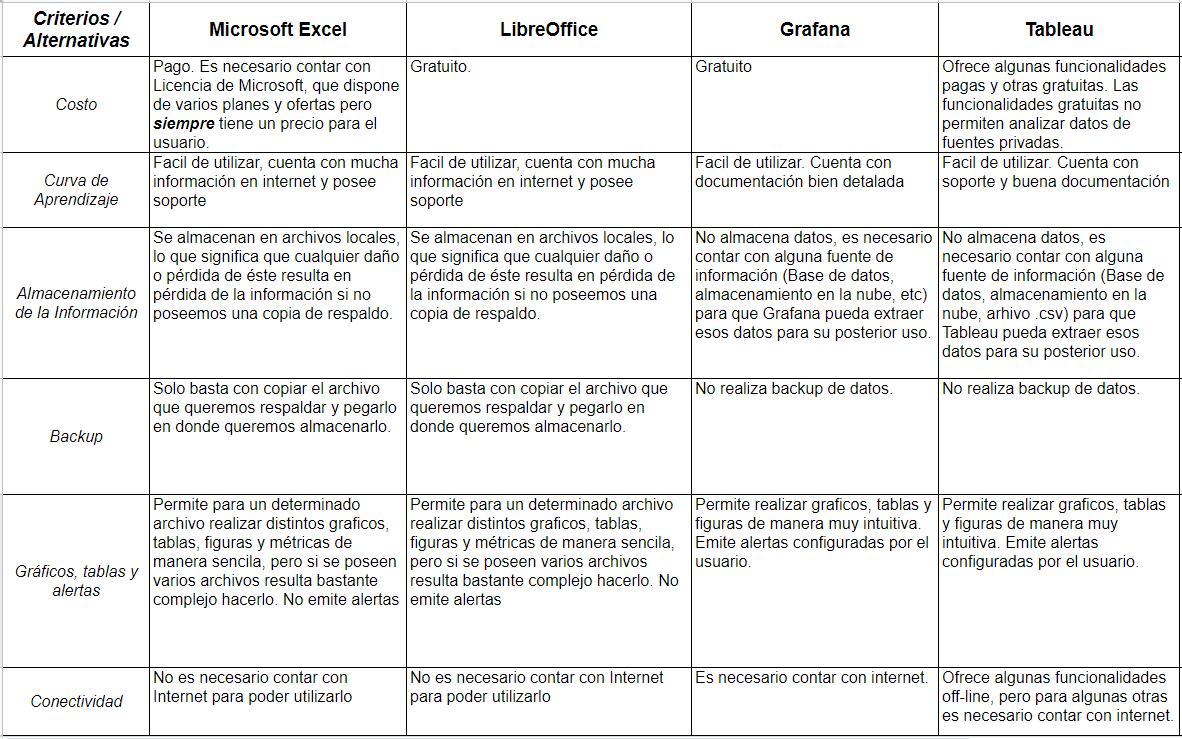
\includegraphics[width=\textwidth]{imagenes/alternativas.png} 
	\caption{Alternativas}
\end{figure}

Además de las alternativas presentadas en el grafico anterior, existen otras aplicaciones web similares como chart.io, klipfolio.com, qlik.com, entre otras pero todas ellas son pagas. \\


Se puede concluir entonces, que no se han detectado alternativas gratuitas y/o herramientas que favorezcan y ayuden al seguimiento de los programas de inclusión.\\


\section*{\underline{METODOLOGÍA}}
Para comenzar se procederá al estudio general de los distintos programas de formación tecnológica para la inclusión de la mujer y se hará un relevamiento de la información disponible de los cursos anteriores de este programa para poder identificar qué datos serían de interés a la hora de ingresarlos al sistema y qué información debería proveer el mismo.\\

Luego se seguirá con un análisis de las funcionalidades del sistema para poder hacer el diseño del mismo.\\

Una vez que el diseño esté finalizado, se comenzará la implementación del sistema.\\

Paralelamente, se desarrollarán y ejecutarán pruebas para asegurar el correcto funcionamiento del mismo.\\

Finalmente, se procederá a realizar pruebas del sistema completo intentando imitar lo mejor posible al funcionamiento real del mismo.\\

Para llevar a cabo todas estas actividades se utilizará una metodología Ágil, en este caso Scrum.\\

Se utilizarán iteraciones llamadas Sprints que tendrán una duración preestablecida de entre 2 y 4 semanas, logrando con esto obtener una retroalimentación continua y rápida del desarrollo del sistema.\\

Para la organización y planificación de las tareas se utilizará el sistema de Trello con su versión FREE. \\

Para realizar las actividades requeridas para la implementación del sistema se definirán tareas semanalmente apoyándose en el tablero de SCRUM que proporciona el sistema Trello. Estas tareas se definirán y dividirán entre los dos estudiantes encargados de realizar el Trabajo Final de Grado.\\

Durante la implementación del sistema se realizarán tres tipos de pruebas paralelamente para asegurar el correcto funcionamiento del mismo:

\begin{itemize}
	\item Pruebas unitarias.
	\item Pruebas de integración.
	\item Pruebas funcionales.\\
\end{itemize}

El equipo estará formado por los siguientes roles:
\begin{itemize}
	\item Scrum Master: Será rotativo entre los dos estudiantes encargados de realizar el proyecto.
	\item Product Owner: Será la Directora de Tesis Sofia Perez.
	\item Sprint Team: Estará compuesto por los dos estudiantes encargados de realizar el proyecto.\\
\end{itemize}

\section*{\underline{RESUMEN TÉCNICO}}
\begin{figure}[H]
	\centering
	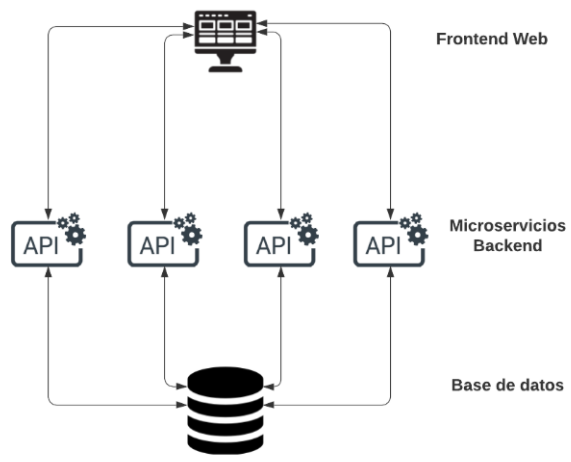
\includegraphics[width=\textwidth]{imagenes/resumen_tecnico.png} 
	\caption{Diagrama de bloques}
\end{figure}

\section*{\underline{PROGRAMACIÓN DE ACTIVIDADES}}

\begin{figure}[H]
	\centering
	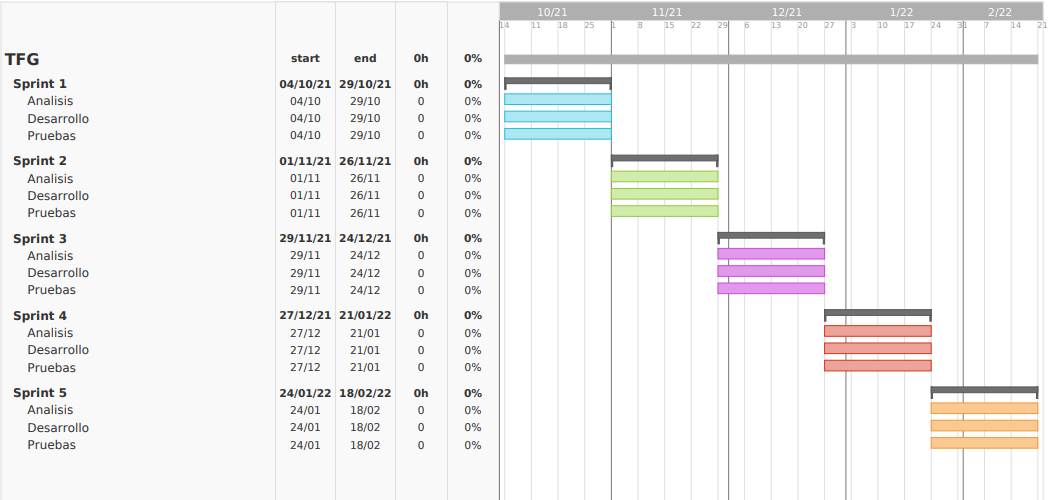
\includegraphics[width=\textwidth]{imagenes/gantt.png} 
	\caption{Diagrama de Gantt}
\end{figure}


\section*{\underline{PROGRAMACIÓN DE RECURSOS}}
Se utilizarán los siguientes recursos y plataformas de desarrollo:
\begin{itemize}
	\item Dos estaciones de trabajo con macOS Big sur, versión 11.2.3.
	\item Entornos de programación de JetBrains con licencia educativa.
	\item Visual Studio Code.
	\item Trello para el seguimiento de las tareas.
	\item Oracle VirtualBox.
	\item Github como versionador de código.
	\item Jenkins como herramienta de Integración Continua y Despliegue Continuo (CI/CD).
	\item Postman free edition.
\end{itemize}

El producto se desplegará sobre un servidor provisto por el Departamento de Computación e Informática, para publicarlo bajo un subdominio de su página web.\\

\section*{\underline{FACILIDADES REQUERIDAS AL IUA}}
Se hará uso de los equipos e infraestructura disponible en el Departamento de Computación e Informática.\\


\section*{\underline{PRESUPUESTO}}
\begin{enumerate}[(a)]
	\item Estimación de costos de equipamiento a utilizar en el proyecto:\\
Valor de un servidor físico con características necesarias:

		\begin{itemize}
			\item Memoria RAM 16GB DDR4.
			\item Disco duro SATA de 4TB.
			\item Procesador escalable Intel® Xeon® 3204 (6 núcleos, 1,9 GHz, 85 W).
			\item Fuente de alimentación 550w.
			\item Estado: Disponible y provisto por el Depto. de Computación e Informática de la Facultad de Ingeniería del CRUC IUA. Costo: \$0.-.
		\end{itemize}

	\item Estimación de costos de desarrollo:
		\begin{itemize}
			\item Se estima que el costo de desarrollo para realizar este proyecto es de 3600 USD, siendo el valor en hora de trabajo de 20 USD, con un total de 180 horas estimadas.\\
		\end{itemize}
\end{enumerate}

\section*{\underline{FUENTES DE FINANCIAMIENTO}}
No corresponde por tratarse de un trabajo final para obtener el título de grado de la carrera.\\

\section*{\underline{RIESGOS ESPERADOS Y SUPUESTOS ASUMIDOS}}
Los riesos esperados son:
\begin{itemize}
	\item Corte de luz, caída de los dominios del IUA o cualquier otro tipo de incidente que perjudique el dominio en donde estará desplegado el sistema ya que los tesistas no se harán cargo del Hosteo.
	\item Si bien los tesistas no son expertos en el dominio, sí lo es su Directora de tesis.\\
\end{itemize}

Los supuestos asumidos son:
\begin{itemize}
	\item Los equipos provistos por el CRUC IUA estarán disponibles desde la fecha de inicio del proyecto.
	\item El equipo del proyecto UNDEX estará disponible para brindar la información necesaria y requerida en el proyecto, así como realizar pruebas y toda actividad derivada de la metodología de desarrollo empleada.\\
\end{itemize}


\section*{\underline{INVERSIÓN REQUERIDA}}
Los tesistas harán uso de equipos e infraestructura disponible en el Departamento de Computación e Informática y aporte de equipos propios.
\begin{itemize}
	\item Servidores (CRUC IUA).
	\item 2 estaciones de trabajo personales (Estudiantes).\\
\end{itemize}

\section*{\underline{PROYECCIÓN DE COSTOS DE OPERACIÓN Y MANTENIMIENTO}}
El sistema se desplegará en un servidor Físico por lo cual los costos de operación y mantenimiento serán los relacionados a los gastos de Luz e Internet que serán a cargo del IUA. \\

La forma en la que será desplegado el sistema en este servidor será la siguiente:
\begin{itemize}
	\item Los microservicios que componen el sistema estarán desplegados con la ayuda de la tecnología de Docker y alguna herramienta para la gestión de estos contenedores.
	\item En cuanto a la base de datos, se utilizará una instalación nativa de MySQL en el servidor físico.
	\item En el caso de necesitar de algún otro servicio que no sea de persistencia de datos se utilizará también la estrategia de despliegue en un contenedor de Docker.
	\item En el caso de necesitar algún otro servicio de persistencia de datos se procederá a utilizar la misma estrategia que con la base de datos MySQL, es decir, se instalará de manera nativa en el servidor.\\
\end{itemize}

Como alternativa se evaluó la opción de desplegar el sistema utilizando algún proveedor en la nube. En este caso se optó por Amazon Web Services por ser uno de los más conocidos y confiables. La sugerencia de despliegue utilizando Amazon Web Services es la siguiente: \\

\begin{figure}[H]
	\centering
	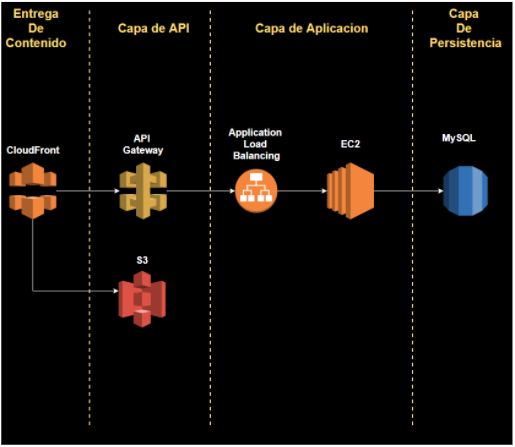
\includegraphics[width=\textwidth]{imagenes/aws_archi.png} 
	\caption{Diagrama de despliegue de microservicios en Amazon Web Services.}
\end{figure}

Esto es una típica implementación de una arquitectura de microservicios utilizando Amazon Web Services pero el costo mensual para poder funcionar es de alrededor 1100 dólares. Este es un costo aproximado ya que para tener una idea más acertada se necesitaría conocer información acerca del uso del sistema como podría ser el volumen de datos que van a ser guardados en la base de datos o la cantidad de tráfico web a la que el sistema será sometido.\\

\section*{\underline{ANÁLISIS DE VIABILIDAD COMERCIAL}}
No corresponde dado que se enmarca en un proyecto UNDEX.\\


\section*{\underline{ANÁLISIS FINANCIERO}}
No corresponde dado que se trata de un trabajo final de carrera.\\
%\footnote{https://www.pagina12.com.ar/325647-software-el-pais-buscara-cuadruplicar-los-puestos-de-trabajo}

\section*{\underline{ESTUDIO AMBIENTAL}}
La elección de un servidor local o en la nube trae impacto ambiental negativo.\\

Mantener toda la información en la nube da la posibildad de no tener que preocuparse por perder y/o procesar información ya que los proveedores de servicios en la nube permiten hacerlo desde cualquier lugar pero esto significa tener la información en datacenters compuestos de miles de servidores que utilizan una cantidad de energía inmensa. Para mantener estos edificios se necesitan kilómetros de fibra óptica e infraestructura que requieren energía en el camino. En el centro, los datos se almacenan varias veces en discos duros, y la actividad constante de todos esos discos genera mucho calor, lo que requiere aires acondicionados que consumen mucha energía para proteger el equipo del sobrecalentamiento.\\
Además, los proveedores de servicios en la nube generan toneladas de desechos electrónicos, aunque algunos de estos proveedores, como Microsoft, están planeando proyectos de reciclaje y redistribuición de los servidores y componentes degradados o en desuso.
\\

Mantener un servidor local, permite controlar de manera más eficiente el uso de la energía y de los componentes, pero no se tiene la ventaja que provee la nube en el procesamiento y almacenamiento de los datos.\\




\section*{\underline{ESTUDIO SOCIAL}}
La industria tecnológica y de desarrollo de software ha tenido un gran crecimiento en los últimos años. La Argentina no es ajena a este proceso: Actualmente la industria del software posee alrededor de 115.000 empleos y se proyecta para el año 2030 unos 500.000 en total o incluso más \textbf{\cite{EmpleosUltAnios}}(Matias K, 2021).\\

En una industria en pleno crecimiento, la inserción de la mujer sigue presentando desafíos:
\begin{itemize}
	\item Aunque en los últimos 15 años se duplicó la participación de mujeres en la industria de IT, todavía la brecha frente a la participación de hombres en esta misma industria es muy grande (70\% hombres, 30\% mujeres).  \textbf{\cite{DuplMujeres}}(Mujeres en la industria del software, 2020)
	\item Solo el 30\% de los estudiantes de carreras de Ciencia, Tecnología, Ingeniería y Matemática (CTIM) que se registran en universidades públicas y privadas son mujeres. \textbf{\cite{MujeresCtim}}(Ana inés \& Cecilia, 2019)\\
\end{itemize}

En adición, la industria de Software es una de las pocas que ha mantenido su crecimiento durante los últimos años y posee uno de los mejores salarios en Argentina.\\

La brecha de género afecta también a la innovación y al crecimiento tanto del campo tecnológico como el desarrollo económico y social de un país. Los programas de inclusión vienen a tratar de disminuir esa brecha de género en tecnología, acercando experiencias formativas a mujeres adolescentes.\\

Es de suma importancia poder tener la posibilidad de realizar un seguimiento de cada alumno que hace estos programas de inclusión para poder sacar conclusiones, métricas y tomar decisiones con el fin de mejorar estas experiencias y por qué no , aumentar la cantidad de mujeres en el rubro de la tecnología. \\

\section*{\underline{EVALUACIÓN ECONÓMICA}}
No corresponde dado que se trata de un trabajo final de carrera.
